\chapter{Topic Service}
\section{Abstract}
The topic micro-service is a large component that handles subtopics, topics, and calendar models. The original monolith had each model separate along with a controller and service for each respectively. We broke down the code from the original monolith by the models, however, the topic and subtopic models were similar enough to merge them into one micro-service. By doing this, we reduced the number of overall micro-services we had as well as the internal service communication that would have had to have taken place. The calendar model was not originally found within the monolith, so we decided to simply add the routes to the topic micro-sevice, since the calendar is only composed of a topic and subtopic.

\section{Service Architecture}

\begin{figure}[htp]
\centering
\includegraphics[width=18cm]{images/topic-package}
\includegraphics[width=18cm]{images/topic-class}
\caption{Topic Service infrastructure}
\label{fig:lion}
\end{figure}


\begin{figure}[htp]
\centering
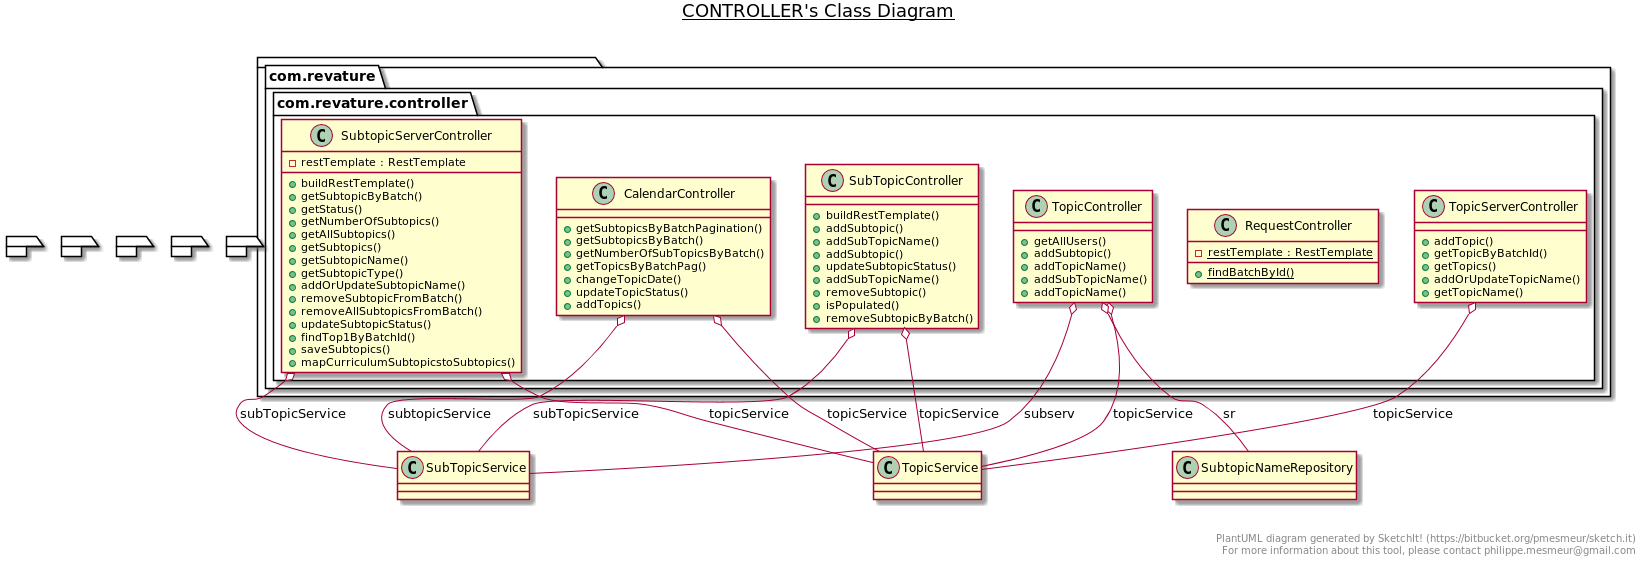
\includegraphics[width=5cm]{images/Topiccontroller}
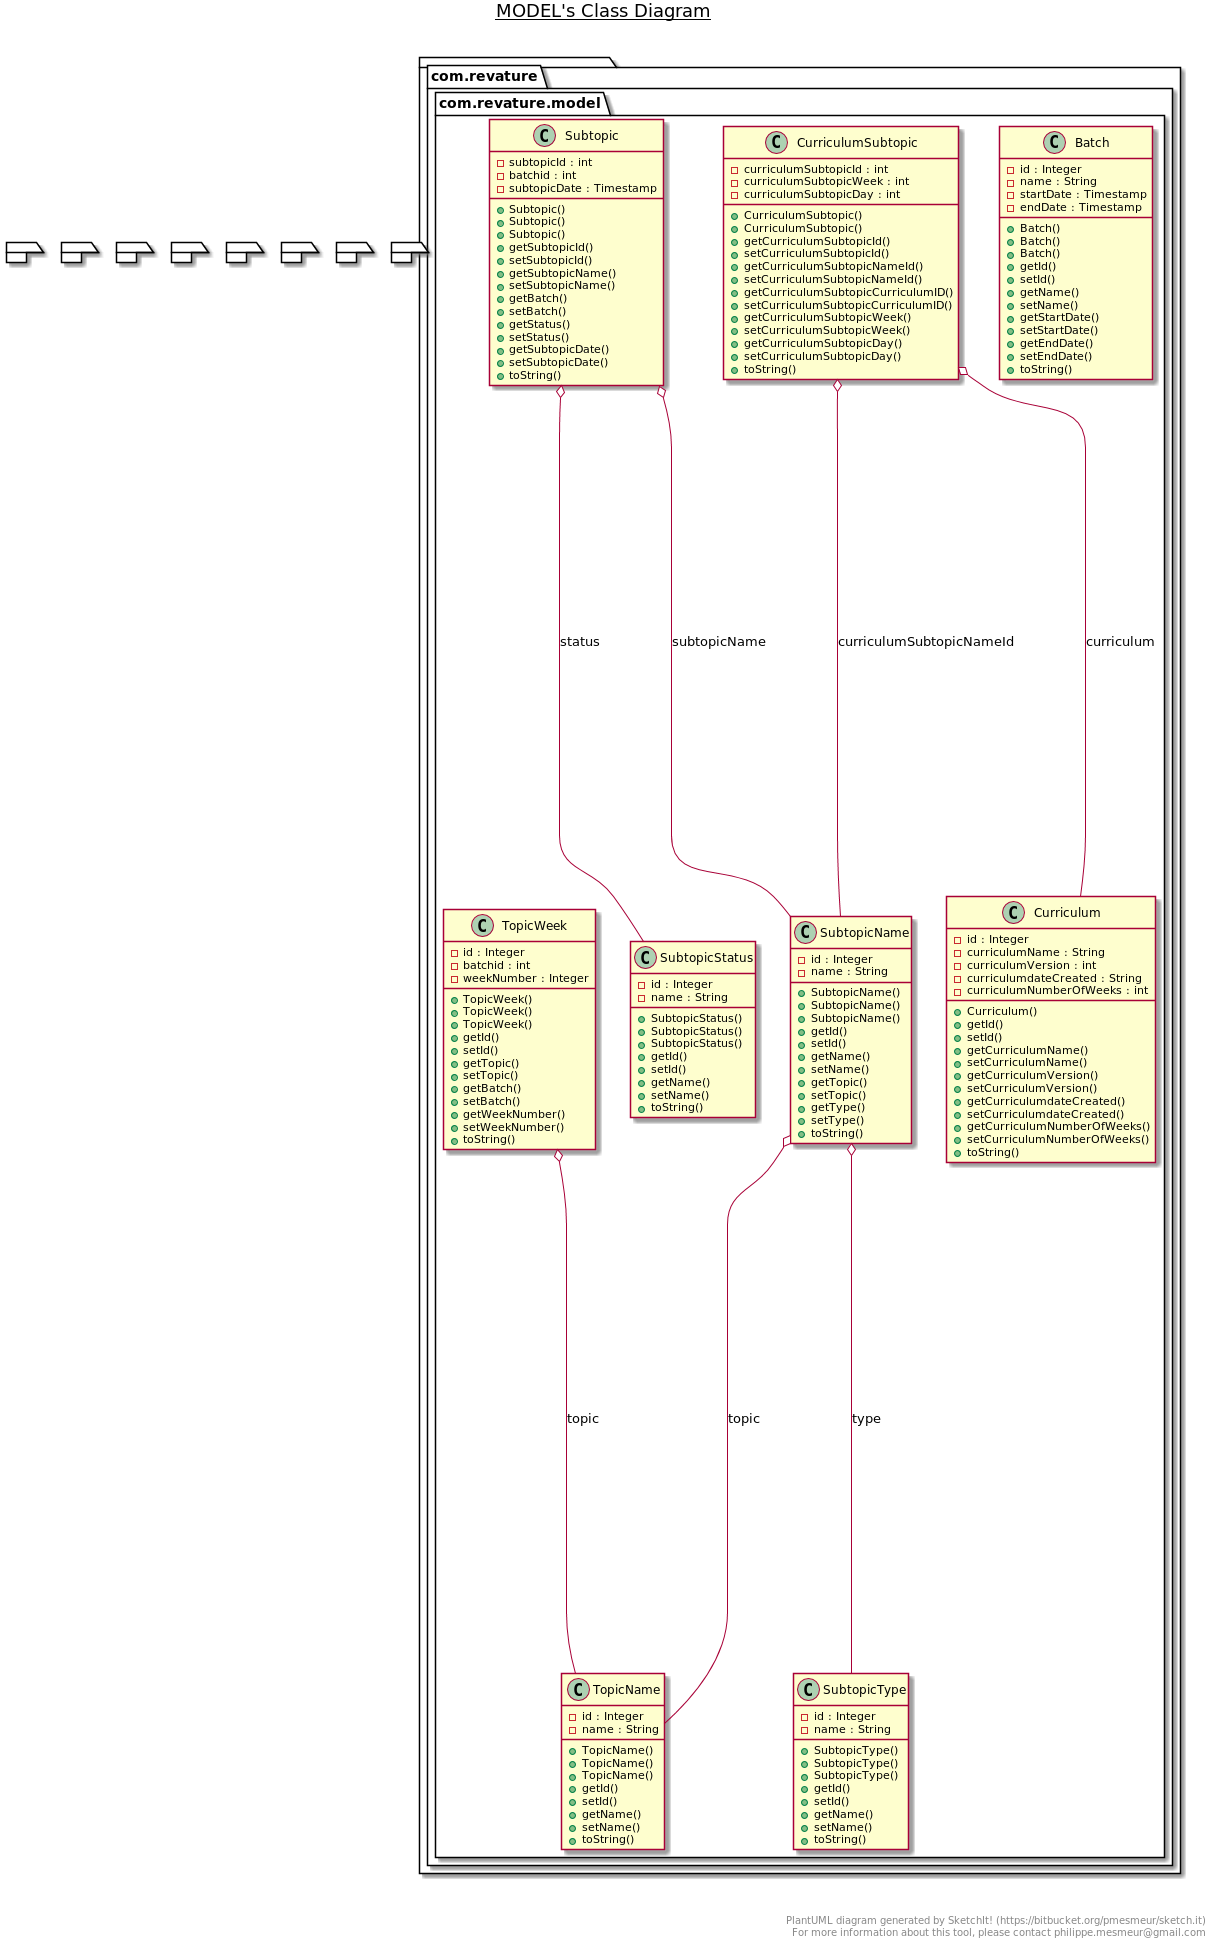
\includegraphics[width=5cm]{images/Topicmodel}
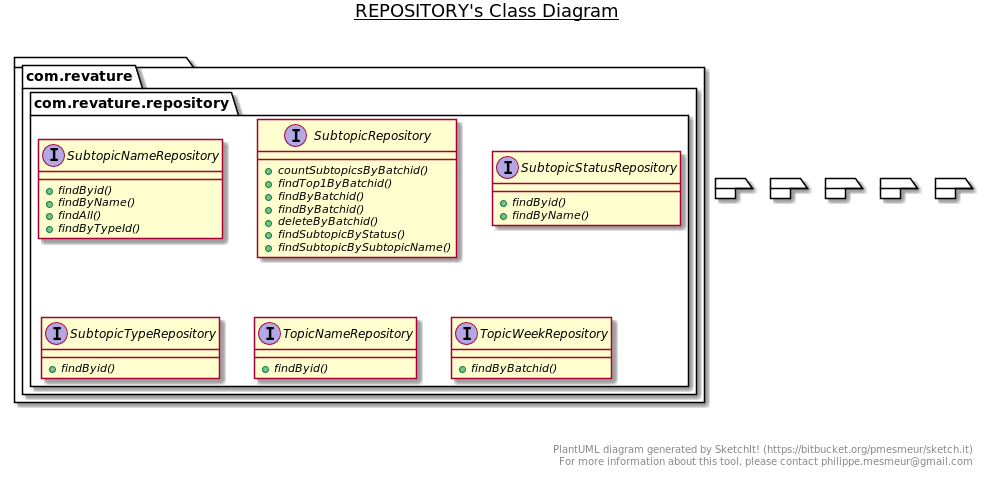
\includegraphics[width=5cm]{images/Topicrepository}
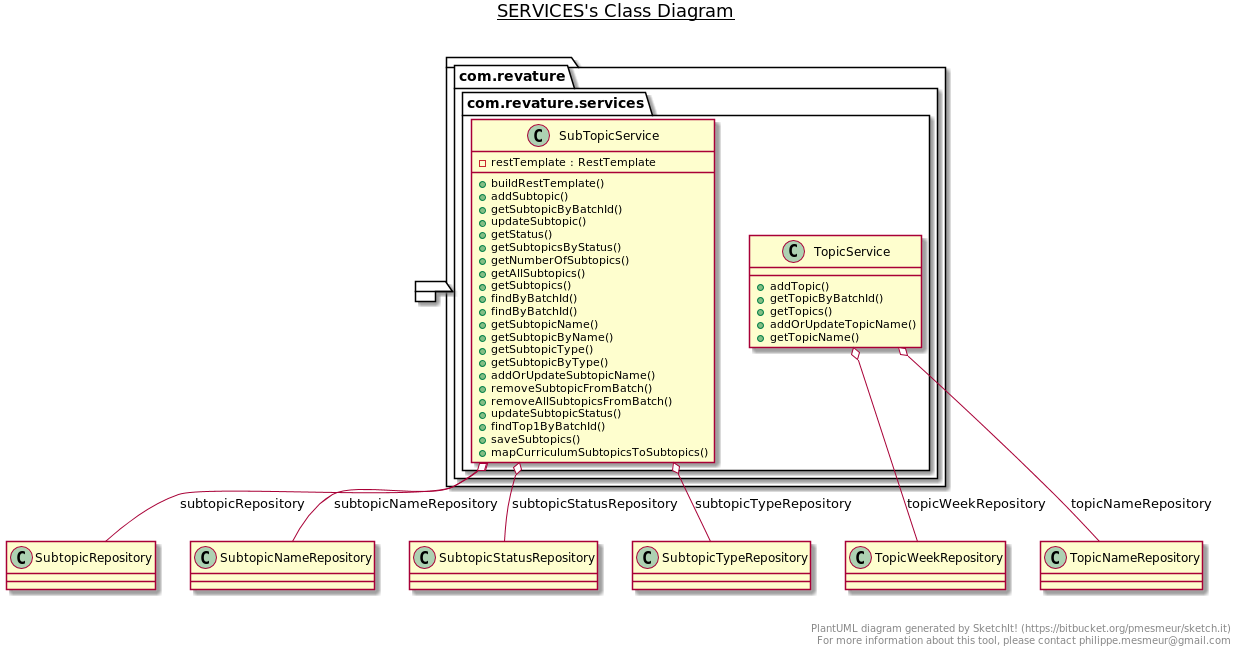
\includegraphics[width=5cm]{images/Topicservices}
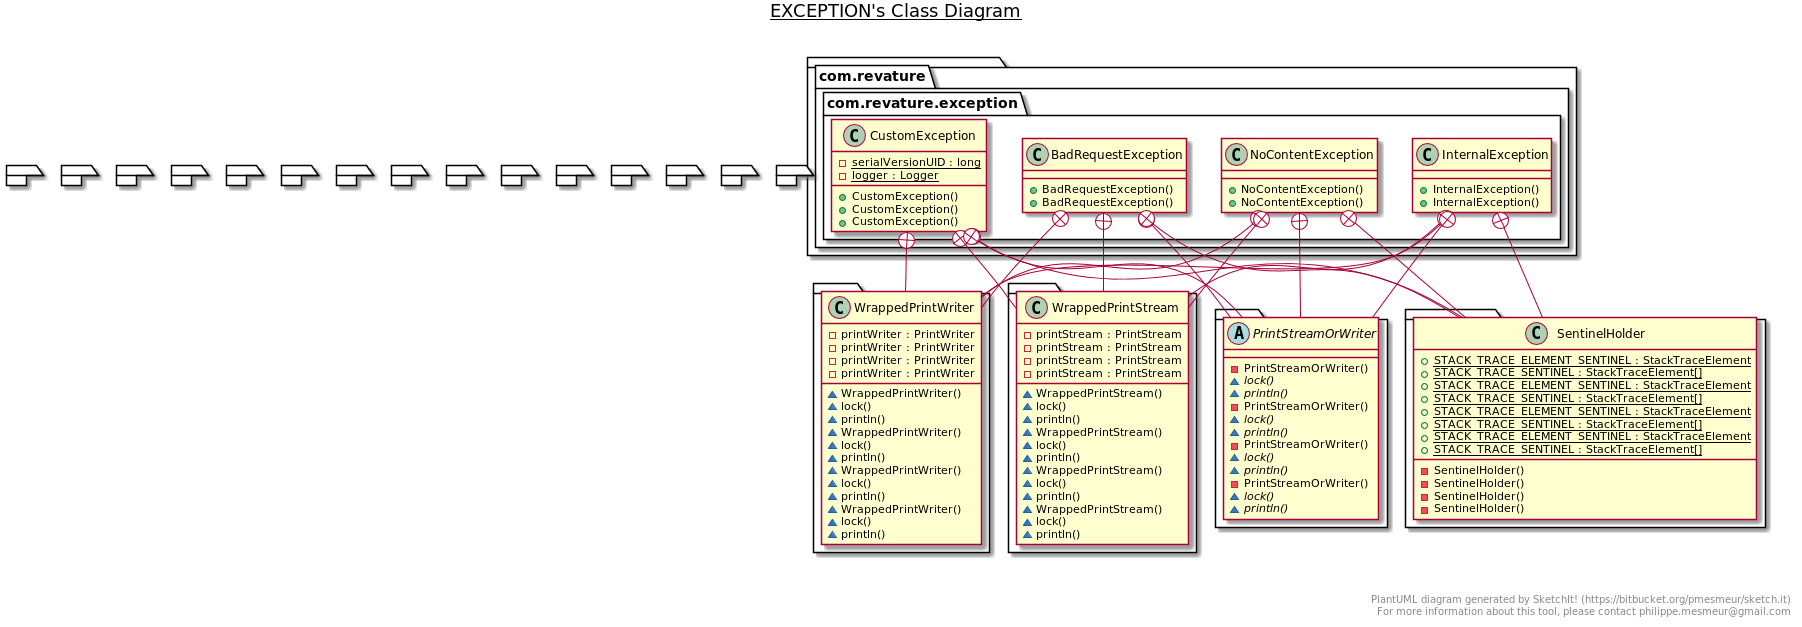
\includegraphics[width=5cm]{images/Topicexception}
\caption{Topic Service Hierarchy}
\label{fig:lion}
\end{figure}